\documentclass[]{article}
\usepackage{lmodern}
\usepackage{fancyhdr}
\usepackage{graphicx}
\pagestyle{fancy}
\rhead{Specyfikacja implementacyjna w Javie: jaguar}
\usepackage{amssymb,amsmath}
\usepackage[utf8]{inputenc}
\usepackage[english]{babel}
\usepackage{lastpage}
\usepackage{amsmath,amscd}
\usepackage[all,cmtip]{xy}
\usepackage{ifxetex,ifluatex}
\usepackage{fixltx2e} % provides \textsubscript
\ifnum 0\ifxetex 1\fi\ifluatex 1\fi=0 % if pdftex
  \usepackage[T1]{fontenc}
  \usepackage[utf8]{inputenc}
\else % if luatex or xelatex
  \ifxetex
    \usepackage{mathspec}
  \else
    \usepackage{fontspec}
  \fi
  \defaultfontfeatures{Ligatures=TeX,Scale=MatchLowercase}
\fi
% use upquote if available, for straight quotes in verbatim environments
\IfFileExists{upquote.sty}{\usepackage{upquote}}{}
% use microtype if available
\IfFileExists{microtype.sty}{%
\usepackage[]{microtype}
\UseMicrotypeSet[protrusion]{basicmath} % disable protrusion for tt fonts
}{}
\PassOptionsToPackage{hyphens}{url} % url is loaded by hyperref
\usepackage[unicode=true]{hyperref}
\hypersetup{
            pdftitle={Specyfikacja implementacyjna generatora i analizatora grafów: jaguar},
            pdfauthor={Kuźmicki Maciej, Skiba Szymon},
            pdfborder={0 0 0},
            breaklinks=true}
\urlstyle{same}  % don't use monospace font for urls
\usepackage{multicol}
\IfFileExists{parskip.sty}{%
\usepackage{parskip}
}{% else
\setlength{\parindent}{0pt}
\setlength{\parskip}{6pt plus 2pt minus 1pt}
}
\setlength{\emergencystretch}{3em}  % prevent overfull lines
\providecommand{\tightlist}{%
  \setlength{\itemsep}{0pt}\setlength{\parskip}{0pt}}
\setcounter{secnumdepth}{0}
% Redefines (sub)paragraphs to behave more like sections
\ifx\paragraph\undefined\else
\let\oldparagraph\paragraph
\renewcommand{\paragraph}[1]{\oldparagraph{#1}\mbox{}}
\fi
\ifx\subparagraph\undefined\else
\let\oldsubparagraph\subparagraph
\renewcommand{\subparagraph}[1]{\oldsubparagraph{#1}\mbox{}}
\fi
% set default figure placement to htbp
\makeatletter
\def\fps@figure{htbp}
\makeatother
\title{Specyfikacja implementacyjna generatora i analizatora grafów: \texttt{jaguar}}
\author{Kuźmicki Maciej, Skiba Szymon}
\date{11.05.2022}
\begin{document}
\maketitle
\thispagestyle{fancy}
\section{Informacje ogólne}\label{header-n231}
\cfoot{Page \thepage \hspace{1pt} of \pageref{LastPage}}
Program \texttt{jaguar} zostanie napisany w języku Java (Java SE 8) w programie \texttt{IntelliJ IDEA}. Do utworzenia graficznego interfejsu użytkownika zostanie wykorzystany pakiet \texttt{Java FX}. Aby zapewnić przenośność kodu program będzie stworzony z pomocą oprogramowania \texttt{Maven}.  Wszystkie kody źródłowe programu umieszczane będą na zdalnym repozytorium w systemie \texttt{projektor} z wykorzystaniem systemu kontroli wersji \texttt{git}. Commit'y będą zawierały infomarcje o tym, co zostało dodane do kodu, bądź w nim zmienione. Do napisania programu zostaną użyte następujące klasy:
\begin{itemize}
\item
\texttt{java.util.ArrayDeque} - w celu skorzystania z kolejki typu FIFO;
\item
\texttt{java.util.ArrayList} - do korzystania z dynamicznych tablic przechowujących zmienne bądź obiekty innych klas;
\item
\texttt{java.util.Random} - do generowania liczb losowych;
\item
\texttt{java.util.Locale} - aby ustawić domyślny format liczb zmiennoprzecinkowych;
\item
\texttt{java.util.Scanner} - do wczytywania danych z pliku.
\end{itemize}


\section{Zastosowane algorytmy i przechowywanie grafu}\label{header-n233}
\begin{itemize}
\item
\texttt{Jaguar} do sprawdzenia spójności danego grafu będzie wykorzystywał algorytm BFS. Polega on na dodaniu do kolejki wierzchołka startowego a następnie na dodawaniu do niej wszystkich sąsiadów wierzchołka znajdującego się na początku kolejki. Po dodaniu wierzchołka do kolejki zaznaczamy w specjalnie stworzonej tablicy, że dany wierzchołek został odwiedzony. Czynności powtarzamy dopóki kolejka będzie zawierała jakieś elementy.
\item
Do wyznaczenia najkrótszej ścieżki pomiędzy dwoma dowolnymi wierzchołkami zostanie wykorzystany algorytm Dijkstry. Jedynym warunkiem wymaganym, aby algorytm ten zadziałał jest to, żeby wagi krawędzi były nieujemne. Wyznacza on odległości do każdego wierzchołka z wierzchołka startowego. W każdym przejściu z wierzchołka do wierzchołka wybierany jest taki, do którego droga jest najkrótsza, analizuje wtedy krawędzi wychodzące z tego wierzchołka i jeśli koszty tych są mniejsze od aktualnego kosztu dotarcia do danego wierzchołka to ustawia dany wierzchołek jako poprzednik wierzchołka, do którego prowadzi ta krawędź.
\item
Graf będzie przechowywany w pamięci komputera za pomocą listy sąsiedztwa. Zostanie ona zaimplementowana za pomocą dwuwymiarowej \texttt{ArrayList'y} przechowującej obiekty klasy \texttt{Neighbor}.

\end{itemize}

\section{Podział na klasy}\label{header-n279}
Program \texttt{jaguar} zostanie podzielony na następujące klasy:
\begin{itemize}
\item
\texttt{Main.java} - klasa zawierająca funkcję main, jej zadaniem jest zintegrowanie funkcjonalności interfejsu graficznego z odpowiednimi klasami;
\item
\texttt{Bfs.java} -  klasa odpowiedzialna za algorytm przeszukiwania grafu wszerz (BFS), jej zadaniem jest poinformowanie użytkownika, czy dany graf jest spójny, zawiera następujące metody:
\begin{itemize}
\item
\texttt{getResult()} - pozwala nam na uzyskanie wyniku działania tej klasy, zwraca zmienną typu boolean;
\item
\texttt{setResult()} - pozwala konstruktorowi na dostęp do prywatnej zmiennej typu boolean z informacją o wyniku w celu ustawienia jego wartości na \texttt{true} albo \texttt{false}, nic nie zwraca;
\item
\texttt{Bfs()} - metoda ta jest konstruktorem, przyjmuje ona obiekt innej klasy typu \texttt{Graf}, jest odpowiedzialna za sprawdzenie spójności przesłanego do niej grafu, zawiera implementacje algorytmu \texttt{BFS}.
\end{itemize} 
\item
\texttt{Neighbor.java} - klasa odpowiedzialna za przechowanie informacji o konkretnym sąsiedzie danego wierzchołka, zawiera następujące metody:
\begin{itemize}
\item
\texttt{getDestination()} - pozwala na uzyskanie informacji o numerze konkretnego sąsiada danego wierzchołka, zwraca wartość typu \texttt{Integer};
\item
\texttt{getWeight()} - pozwala na uzyskanie informacji o wadze przejścia do konkretnego sąsiada danego wierzchołka, zwraca wartość typu \texttt{Double}; 
\item
\texttt{Neighbor()} - metoda ta jest konstruktorem, przyjmuje informacje o numerze konkretnego sąsiada danego wierzchołka oraz o wadze przejścia do niego, przypisuje te informacje do prywatnych zmiennych. 
\end{itemize}
\item
\texttt{Graf.java} - klasa odpowiedzialna za wczytanie grafu z pliku do pamięci komputera do dwuwymiarowej \texttt{ArrayList'y} przechowującej obiekty klasy \texttt{Neighbor} oraz za zapisanie grafu do pliku, zawiera następujące metody: 
\begin{itemize}
\item
\texttt{AllocateMemoryForEdges()} - metoda ta alokuje przestrzeń w pamięci komputera dla grafu;
\item
\texttt{getRow()} - metoda ta zwraca informację o liczbie wierszy danego grafu;
\item
\texttt{getColumn()} - metoda ta zwraca informację o liczbie kolumn danego grafu;
\item
\texttt{setRow()} - metoda ta pozwala zapisać informację o liczbie wierszy do prywatnej zmiennej;
\item
\texttt{setColumn()} - metoda ta pozwala zapisać informację o liczbie kolumn do prywatnej zmiennej;
\item
\texttt{getNeighbors()} - metoda ta zwraca dwuwymiarową \texttt{ArrayList'e} przechowującą obiekty klasy \texttt{Neighbor};
\item
\texttt{ReadFromFile()} - metoda ta przyjmuje nazwę pliku, z którego ma czytać informację o sąsiadach kolejnych wierzchołków, zajmuję się przeczytaniem tych wierzchołków oraz zapisaniem ich do dwuwymiarowej \texttt{ArrayList'y}, nic nie zwraca;
\item
\texttt{AddEdgeForGraf()} - metoda ta przyjmuje informację o sąsiedzie konkretnego wierzchołka oraz wadze przejścia do niego, tworzy obiekt klasy \texttt{Neighbor} a następnie go zwraca;
\item
\texttt{WriteToFile()} - metoda ta przyjmuje nazwę pliku, do którego ma zapisać informacje o sąsiadach kolejnych wierzchołków danego grafu, a następnie zapisuje je do tego pliku, nic nie zwraca;
\item
\texttt{PrintGraf()} - metoda ta jest odpowiedzialne za wyświetlanie grafu na ekranie.
\end{itemize}
\item
\texttt{Generator.java} - klasa ta odpowiedzialna jest za wygenerowanie grafów:
\begin{itemize}
\item
\texttt{tlw()} - metoda ta przyjmuje liczbę wierszy, liczbę kolumn oraz zakres liczb, spomiędzy których program ma wygenerować wagi, zwraca obiekt typu \texttt{Graf} zawierający krawędzie pomiędzy każdymi dwoma dowolnymi wierzchołkami;
\item
\texttt{bf()} - metoda ta przyjmuje liczbę wierszy, liczbę kolumn oraz zakres liczb, spomiędzy których program ma wygenerować wagi, zwraca obiekt typu \texttt{Graf}. Losowo generuje połączenia pomiędzy wierzchołkami z prawdopodobieństwem 0.7.
\end{itemize} 
\item
\texttt{Dijkstra.java} - klasa ta odpowiedzialna jest za wygenerowanie ścieżki i najkrótszej odległości pomiędzy dwoma wierzchołkami grafu:
\begin{itemize}
\item
\texttt{setPath()} - metoda ta pozwala modyfikować zmienna przechowującą najkrótszą ścieżkę.;
\item
\texttt{getPath()} - metoda ta pozwala odczytywać zmienna przechowującą najkrótszą ścieżkę;
\item
\texttt{setLength()} - metoda ta pozwala modyfikować zmienna przechowującą długość najkrótszej ścieżki; 
\item
\texttt{getLength()} - metoda ta pozwala odczytywać zmienna przechowującą długość najkrótszej ścieżki; 
\item
\texttt{Dijkstra()} - metoda ta jest konstruktorem, przyjmuje numery  wierzchołka startowego i wierzchołka końcowego. Znajduje najkrótszą ścieżkę i jej długość. 
\end{itemize} 
\end{itemize}
\section{Wykorzystanie przez GUI opisanych klas}\label{header-n281}
\begin{center}
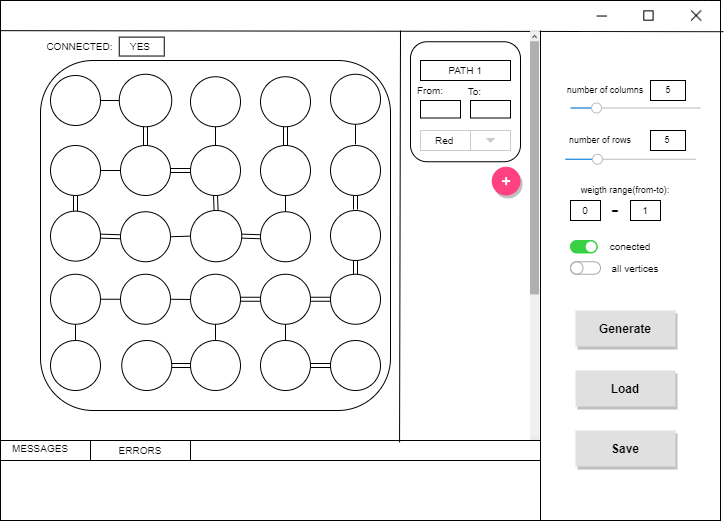
\includegraphics[scale=0.3]{gui_jimp.drawio}
\end{center}
\begin{center}
(rys. 1 Projekt GUI)
\end{center}
\begin{itemize}
\item
\texttt{przycisk GENERATE} - po ustawieniu parametrów na w menu kontekstowym po prawej wywołuje odpowiednio metodę \texttt{bf()} lub \texttt{tlw()} z klasy \texttt{Generate} oraz metodę \texttt{PrintGraf()} z klasy \texttt{Graf}.
\item
\texttt{przycisk LOAD} - wywołuje metodę \texttt{ReadFromFile()} oraz metodę \texttt{PrintGraf()} z klasy \texttt{Graf}.
\item
\texttt{przycisk SAVE} - wywołuje metodę \texttt{WriteToFile()}.
\item
\texttt{przycisk "PLUS" lub zaznaczenie ścieżki na grafie} - wywołuje metodę \texttt{Dijkstra()} i wyświetla korzystając z metod \texttt{getPath()}, \texttt{getLength()} wyświetla w oknie dialogowym ścieżkę i jej długość.

\end{itemize} 


\section{Opis testów programu}\label{header-n281}
W celu sprawdzenia, czy program działa poprawnie napisane zostaną testy. Każdy klasa będzie miała swoją klasę o identycznej nazwie z dopiskiem \texttt{Test}. Zostaną w niej zaimplementowane testy poszczególnych metod. Zostanę napisane one z pomocą oprogramowania \texttt{JUnit}. 



\end{document}
